
\section{Infomax tuning curves for a given stimulus distribution}\label{sec:laughlin}

Let a stimulus $S$ have distribution $P_S$, and let a neuron map it to an expected spike count $r(S)$ in one counting window, with
$\lambda\le r(s)\le\lambda+A$; here $\lambda$ is the spontaneous count and $A$ the peak count above it. The response is
$Y\,|\,S=s\sim\mathrm{Poisson}(r(s))$. The tuning curve $r$ is the design variable and $P_S$ is fixed, as in Barlow's and Laughlin's
formulation of efficient coding. Let $C(A,\lambda)$ be the capacity of the Poisson channel with input in $[\lambda,\lambda+A]$, the
largest mutual information between rate and count that any distribution of rates in this range can give; for example,
$C(3,0)=0.5944$ nats, or $0.858$ bits per window. Let
$\pi=\sum_{j=1}^{K}w_j\delta_{x_j}$, with weights $w_j$ and mass points $x_1<\dots<x_K$, be its capacity-achieving input: the
distribution of rates that gives probability $w_j$ to the rate $x_j$ and reaches the capacity. Shamai proved that it is unique and has
finitely many mass points~\cite{Shamai1990}. The letter $\pi$ always denotes this distribution; the number $3.14159$ enters only
inside constants of Theorem~\ref{thm:C} and its proof. Write $W_j=w_1+\dots+w_j$ and $W_0=0$.

\begin{proposition}\label{prop:L1}
For every measurable tuning curve $r$ with values in $[\lambda,\lambda+A]$,
\[
I(S;Y)\le C(A,\lambda),
\]
with equality if and only if the law of $r(S)$ is $\pi$. If $P_S$ has a continuous distribution function $F_S$, equality is attained,
and, up to a $P_S$-null set, the nondecreasing maximizer is the staircase
\[
r^*(s)=x_j\qquad\text{for } F_S(s)\in(W_{j-1},W_j],\quad j=1,\dots,K .
\]
Every maximizer takes exactly $K$ values outside a $P_S$-null set.
\end{proposition}

In words: no tuning curve carries more information than the capacity, and a tuning curve reaches it exactly when the rates it
produces have the distribution $\pi$. The law of $r(S)$ is this distribution of produced rates, and a $P_S$-null set is a set of
stimuli of probability zero, on which two tuning curves may differ without any change in information. The count depends on the
stimulus only through the rate, so passing from the stimulus to the rate loses nothing, and the information of the tuning curve is
the information of its rates. To build the nondecreasing one, sort the stimuli by their cumulative probability. Give the lowest
rate $x_1$ to the lowest fraction $w_1$ of stimuli, the next rate $x_2$ to the next fraction $w_2$, and so on up to $x_K$. Any
assignment of the rates to pieces of the stimulus distribution with these probabilities is optimal; the nondecreasing one has the shape
of the rate-level functions recorded in the auditory nerve.

\begin{proof}
Put $X=r(S)$. The count is drawn from the rate alone, so given $X$ the count does not depend on $S$; thus $S\to X\to Y$ is a Markov
chain and $I(S;Y)\le I(X;Y)$. Since $X$ is computed from $S$, also $X\to S\to Y$ is a Markov chain and $I(X;Y)\le I(S;Y)$. Hence
$I(S;Y)=I(X;Y)$. The variable $X$ takes values in $[\lambda,\lambda+A]$, so $I(X;Y)\le C(A,\lambda)$, with equality if and only if the
law of $X$ is a capacity-achieving input, that is $\pi$ by uniqueness. If $F_S$ is continuous, $U=F_S(S)$ is uniform on $(0,1)$. Let
$G$ be the distribution function of $\pi$ and $G^{-1}(u)=\inf\{x:G(x)\ge u\}$ its quantile function. Then $r^*(S)=G^{-1}(U)$ has law $\pi$, so $r^*$ attains
the bound; it is nondecreasing and takes the value $x_j$ exactly when $U\in(W_{j-1},W_j]$. Any maximizer has law $\pi$, a $K$-point
law, so it takes $K$ values almost surely.
\end{proof}

The proposition separates two questions. The stimulus distribution decides where the steps sit, at its quantiles $W_j$; it does not
change their number or their values, which depend only on $A$ and $\lambda$. A staircase shape of the optimal tuning curve was found
numerically for Poisson neurons with a finite coding window~\cite{Nikitin2009}; the proposition derives it for every continuous
stimulus law from the uniqueness and discreteness of $\pi$. Fig~\ref{fig:schematic} shows the construction for a Gaussian stimulus.

\begin{figure}[!ht]
\centering
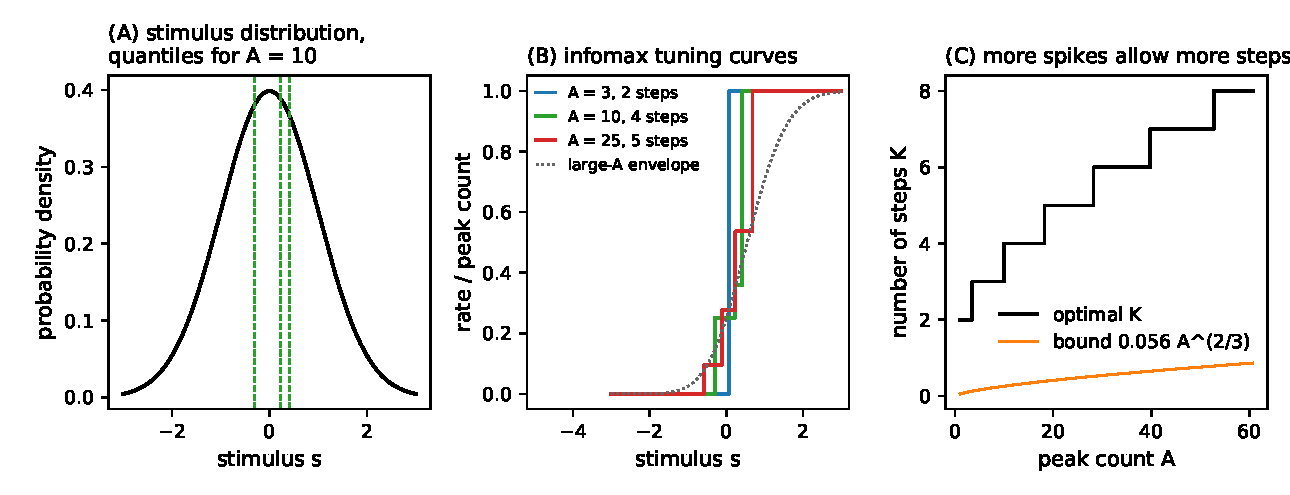
\includegraphics[width=\textwidth]{figs/fig_schematic.pdf}
\caption{\textbf{The infomax tuning curve of a Poisson neuron is a staircase.} (A) A Gaussian stimulus distribution; the three dashed
lines, $W_1$ to $W_3$ from left to right, mark the stimulus values below which the stimulus falls with probability $W_j$; the optimal tuning curve steps
there for peak count $A=10$ and no spontaneous count. (B) The optimal tuning
curves for $A=3$, $10$ and $25$, as a fraction of the peak count, with 2, 4 and 5 steps. Much of the weight of the optimal input sits at the lowest rate,
silence, and at the peak rate, so the inner steps lie close to the middle of the stimulus range; the dotted curve $F_S(s)^2$ is the envelope
that the staircase approaches only for large $A$. (C) The number of steps against the peak count, from numerical solutions of the
capacity problem, with the asymptotic lower bound $0.056\,A^{2/3}$ of Theorem~\ref{thm:C}; at these peak counts the bound lies far
below the number of steps, since it concerns how the number grows for large $A$. All values are computed numerically.}\label{fig:schematic}
\end{figure}

\begin{corollary}\label{cor:L2}
Fix $\lambda\ge0$, and let $K(A,\lambda)$ be the number of mass points of $\pi$ at peak count $A$. Then the infomax tuning curve of
Proposition~\ref{prop:L1} has $K(A,\lambda)$ steps, and $\liminf_{A\to\infty}K(A,\lambda)/A^{2/3}\ge 0.0560$.
\end{corollary}
\begin{proof}
The number of values of $r^*$ is the number of mass points of $\pi$; apply Theorem~\ref{thm:C}, stated in the next section.
\end{proof}

The corollary holds for every fixed spontaneous count, as the fibres have. At the small peak counts of the fibres the bound says
little, and the number of steps is computed numerically, as in Section~\ref{sec:an}.

In the coordinate $2\sqrt r$ the Poisson noise has unit width and the range $[0,A]$ has length $2\sqrt A$, its Fisher length. A count
of distinguishable levels, the Fisher length divided by the width of the noise, therefore grows only like $\sqrt A$. Since
$2/3-1/2=1/6$, the infomax staircase uses more steps than that, by a factor of order $A^{1/6}$ at least. This comparison concerns
large $A$: the constant $0.056$ is small, and at the peak counts of Fig~\ref{fig:schematic}C the bound lies far below the actual
number of steps.

\emph{The large-$A$ limit.} As $A$ grows, the steps become dense. In the limit of small noise the capacity-achieving distribution of
the rate approaches the density proportional to the square root of the Fisher information. The Fisher information of a Poisson
count about its rate $r$ is $1/r$, so this density is proportional to $r^{-1/2}$. McDonnell and Stocks~\cite{McDonnellStocks2008} use this argument to derive the optimal tuning curve as a
nonlinear function of the stimulus distribution function. Under this density $\sqrt r$ is uniform on $[\sqrt\lambda,\sqrt{\lambda+A}]$.
Proposition~\ref{prop:L1} maps the quantiles of the stimulus to the quantiles of this law, so that
\begin{equation}
r(s)\approx\bigl(\sqrt\lambda+(\sqrt{\lambda+A}-\sqrt\lambda)\,F_S(s)\bigr)^2 .\label{eq:envelope}
\end{equation}
Without spontaneous count Eq~\eqref{eq:envelope} becomes $A\,F_S(s)^2$, and it is close to $\lambda+A\,F_S(s)^2$ only when $\lambda$ is small compared with
$A$. This is histogram equalization in the square-root coordinate, the Poisson form of Laughlin's rule. The approximation describes the
envelope of the optimal staircase when $A$ is large and the steps are many. At the peak counts of the rate-level functions of Section~\ref{sec:an},
about 5 to 14 for four fibres in five, the staircase has only a few steps, and the smooth curve is the predicted shape of its envelope. The shape test of Section~\ref{sec:an} checks this envelope, and its
discreteness test checks the number of steps.
